\documentclass[a4paper,14pt]{extarticle}

\usepackage[utf8x]{inputenc}
\usepackage[T1]{fontenc}
\usepackage[russian]{babel}
\usepackage{hyperref}
\usepackage{indentfirst}
\usepackage{here}
\usepackage{array}
\usepackage{graphicx}
\usepackage{grffile}
\usepackage{caption}
\usepackage{subcaption}
\usepackage{chngcntr}
\usepackage{amsmath}
\usepackage{amssymb}
\usepackage{pgfplots}
\usepackage{pgfplotstable}
\usepackage[left=2cm,right=2cm,top=2cm,bottom=2cm,bindingoffset=0cm]{geometry}
\usepackage{multicol}
\usepackage{multirow}
\usepackage{titlesec}
\usepackage{listings}
\usepackage{color}
\usepackage{longtable}
\usepackage{enumitem}
\usepackage{cmap}
\usepackage{tikz}

\usetikzlibrary{shapes,arrows}

\definecolor{green}{rgb}{0,0.6,0}
\definecolor{gray}{rgb}{0.5,0.5,0.5}
\definecolor{purple}{rgb}{0.58,0,0.82}

\lstset{
	language={C},
	inputpath={../},
	backgroundcolor=\color{white},
	commentstyle=\color{green},
	keywordstyle=\color{blue},
	numberstyle=\scriptsize\color{gray},
	stringstyle=\color{purple},
	basicstyle=\small,
	breakatwhitespace=false,
	breaklines=true,
	captionpos=b,
	keepspaces=true,
	numbers=left,
	numbersep=5pt,
	showspaces=false,
	showstringspaces=false,
	showtabs=false,
	tabsize=8,
	frame=single,
}

\renewcommand{\le}{\ensuremath{\leqslant}}
\renewcommand{\leq}{\ensuremath{\leqslant}}
\renewcommand{\ge}{\ensuremath{\geqslant}}
\renewcommand{\geq}{\ensuremath{\geqslant}}
\renewcommand{\epsilon}{\ensuremath{\varepsilon}}
\renewcommand{\phi}{\ensuremath{\varphi}}
\renewcommand{\thefigure}{\arabic{figure}}
\def\code#1{\texttt{#1}}

\titleformat*{\section}{\large\bfseries} 
\titleformat*{\subsection}{\normalsize\bfseries} 
\titleformat*{\subsubsection}{\normalsize\bfseries} 
\titleformat*{\paragraph}{\normalsize\bfseries} 
\titleformat*{\subparagraph}{\normalsize\bfseries} 

\counterwithin{figure}{section}
\counterwithin{equation}{section}
\counterwithin{table}{section}
\newcommand{\sign}[1][5cm]{\makebox[#1]{\hrulefill}}
\newcommand{\equipollence}{\quad\Leftrightarrow\quad}
\newcommand{\no}[1]{\overline{#1}}
\graphicspath{{figs/}}
\captionsetup{justification=centering,margin=1cm}
\def\arraystretch{1.3}
\setlength\parindent{5ex}
\titlelabel{\thetitle.\quad}

\setitemize{itemsep=0em}
\setenumerate{itemsep=0em}

\tikzstyle{startstop} = [
	rectangle,
	align=center,
	rounded corners,
	text width=10em,
	text centered,
	draw=black
]
\tikzstyle{process} = [
	rectangle,
	align=center,
	text width=20em,
	text centered,
	draw=black
]
\tikzstyle{decision} = [
	diamond,
	aspect=4,
	align=center,
	inner sep=0pt,
	text width=10em,
	text centered,
	node distance=5em,
	draw=black
]
\tikzstyle{line} = [
	draw=black,
	thick,
	->,
	>=stealth,
	-latex'
]

\begin{document}

\begin{titlepage}
\begin{center}
	САНКТ-ПЕТЕРБУРГСКИЙ ПОЛИТЕХНИЧЕСКИЙ УНИВЕРСИТЕТ\\ ПЕТРА ВЕЛИКОГО\\[0.3cm]
	\par\noindent\rule{10cm}{0.4pt}\\[0.3cm]
	Институт компьютерных наук и технологий \\[0.3cm]
	Кафедра компьютерных систем и программных технологий\\[4cm]
	
	Отчет по лабораторной работе\\[3mm]
	Дисциплина: <<Технологии компьютерных сетей>>\\[3mm]
	Тема: <<Программирование сокетов протоколов TCP и UDP>>\\[7cm]
\end{center}

\begin{flushleft}
	\hspace*{5mm} Выполнил студент гр. 43501/3  \hspace*{2.5cm}\sign[3cm]\hfill А.Ю. Ламтев\\
	\hspace*{10.4cm} (подпись)\\[3mm]
	\hspace*{5mm} Преподаватель \hspace*{6.0cm}\sign[3cm]\hfill А.В. Зозуля\\
	\hspace*{10.4cm} (подпись)\\[3mm]
	\hspace*{11.1cm} <<\sign[7mm]>> \sign[27mm] \the\year\hspace{1mm} г.
\end{flushleft}

\vfill

\begin{center}
	Санкт-Петербург\\
	\the\year
\end{center}
\end{titlepage}
\addtocounter{page}{1}

\tableofcontents
\listoffigures
\listoftables
\newpage

\section{Задание}

\subsection{Формулировка}

Разработать приложение-сервер <<Удаленный калькулятор>>, позволяющее по запросу выполнять математические операции, и удаленный клиент для сервера.

\subsection{Основные возможности}

Серверное приложение должно реализовывать следующие функции:

\begin{enumerate}
	\item Прослушивание определенного порта
	\item Обработка запросов на подключение по этому порту от клиентов
	\item Поддержка одновременной работы нескольких клиентов через механизм нитей
	\item Приём <<быстрых>> операций с аргументами от клиента. Должны поддерживаться следующие операции: сложение, вычитание, умножение,
деление
	\item Вычисление <<долгих>> математических операций (факториал, квадратный корень) с последующей отложенной посылкой результата клиенту (отдельная операция, инициируемая сервером).
	\item Обработка запроса на отключение клиента
	\item Принудительное отключение клиента
\end{enumerate}

Клиентское приложение должно реализовывать следующие функции:

\begin{enumerate}
	\item Установление соединения с сервером
	\item Посылка операции с аргументами на вычисление
	\item Получение результата вычислений <<быстрых>> операций
	\item Получения результата вычислений <<долгих>> операций
	\item Разрыв соединения
	\item  Обработка ситуации отключения клиента сервером
\end{enumerate}

\subsection{Настройки приложений}

Разработанное клиентское приложение должно предоставлять пользователю настройку IP-адреса или доменного имени удалённого калькулятора и номера порта, используемого сервером. Разработанное серверное приложение должно предоставлять пользователю настройку времени выполнения <<долгих>> операций. 

\subsection{Методика тестирования}

Для тестирования приложений запускается сервер <<Удаленного калькулятора>> и несколько клиентов. В процессе тестирования проверяются основные возможности калькулятора по мгновенному и отложенному выполнению удалённых операций. 

\section{Прикладной протокол}
%Описание форматов команд и ответов (например, в табличном виде: набор и формат команд, размеры полей, сообщения об ошибках). Прикладной протокол не зависит от нижележащего транспортного протокола, а также от языка и технологии программирования.

Разработанный протокол является бинарным, формат сообщения представлен на рис. \ref{fig:calc-prot}.

\begin{figure}[H]
	\centering
	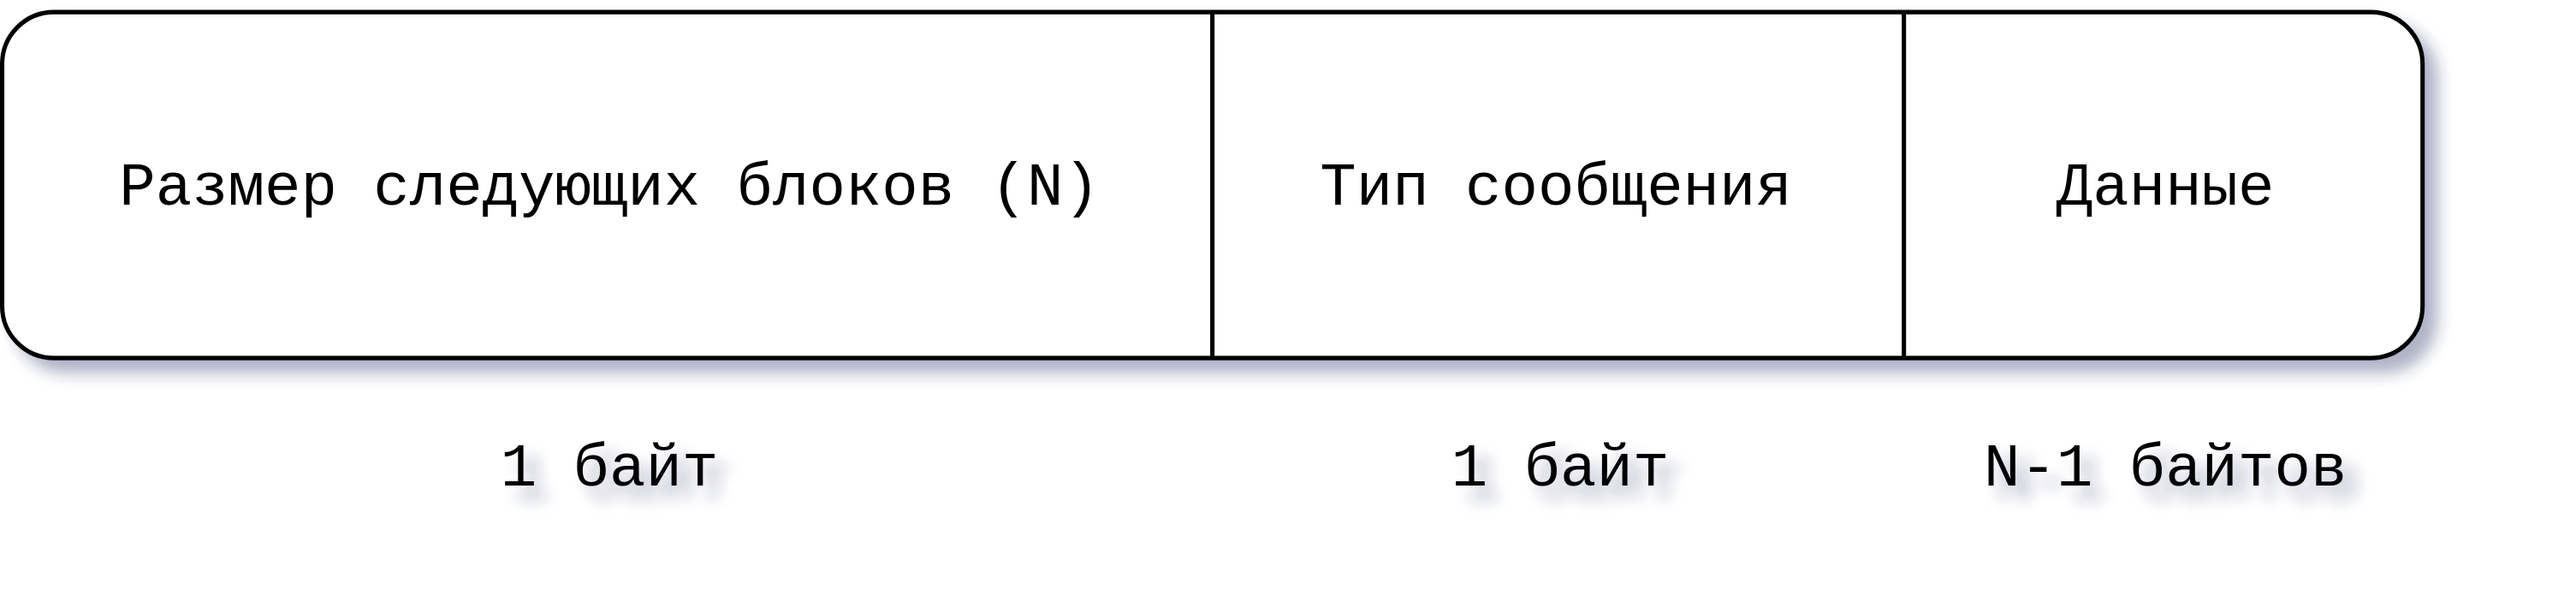
\includegraphics[width=1\textwidth]{CalculatorProtocol}
	\caption{Формат сообщения}
	\label{fig:calc-prot}
\end{figure}

Сообщение разделено на 3 блока:

\begin{enumerate}
	\item Содержит размер следующих блоков в байтах ($N$). Занимает 1 байт
	\item Содержит тип сообщения, который занимает 1 байт
	\item Содержит данные, которые занимают $N-1$ байтов 
\end{enumerate}

В таблице \ref{tab:msg-types} представлены возможные типы сообщений и их бинарное представление.

\begin{table}[H]
\begin{center}
	\caption{Типы сообщений}
	\label{tab:msg-types}
	\def\tabcolsep{10pt}
	\def\arraystretch{1.23}
	\begin{tabular}{|c|c|c|}
		\hline 
		& Тип сообщения & Бинарное представление \\ 
		\hline 
		1 & Математический запрос & $0000\text{ }0000$ \\ 
		\hline 
		2 & Ответ на математический запрос & $0000\text{ }0001$ \\ 
		\hline 
		3 & Управляющий запрос & $0000\text{ }0010$ \\ 
		\hline 
		4 & Ответ на управляющий запрос & $0000\text{ }0011$ \\ 
		\hline
		5 & Запрос, инициируемый сервером & $0000\text{ }0100$ \\ 
		\hline
	\end{tabular} 
\end{center}
\end{table}

Ниже представлен формат данных для каждого типа сообщения:

\begin{enumerate}
	\item \textbf{Математический запрос}.
	
	Формат данных приведен на рис. \ref{fig:math-req}
	
	\begin{figure}[H]
		\centering
		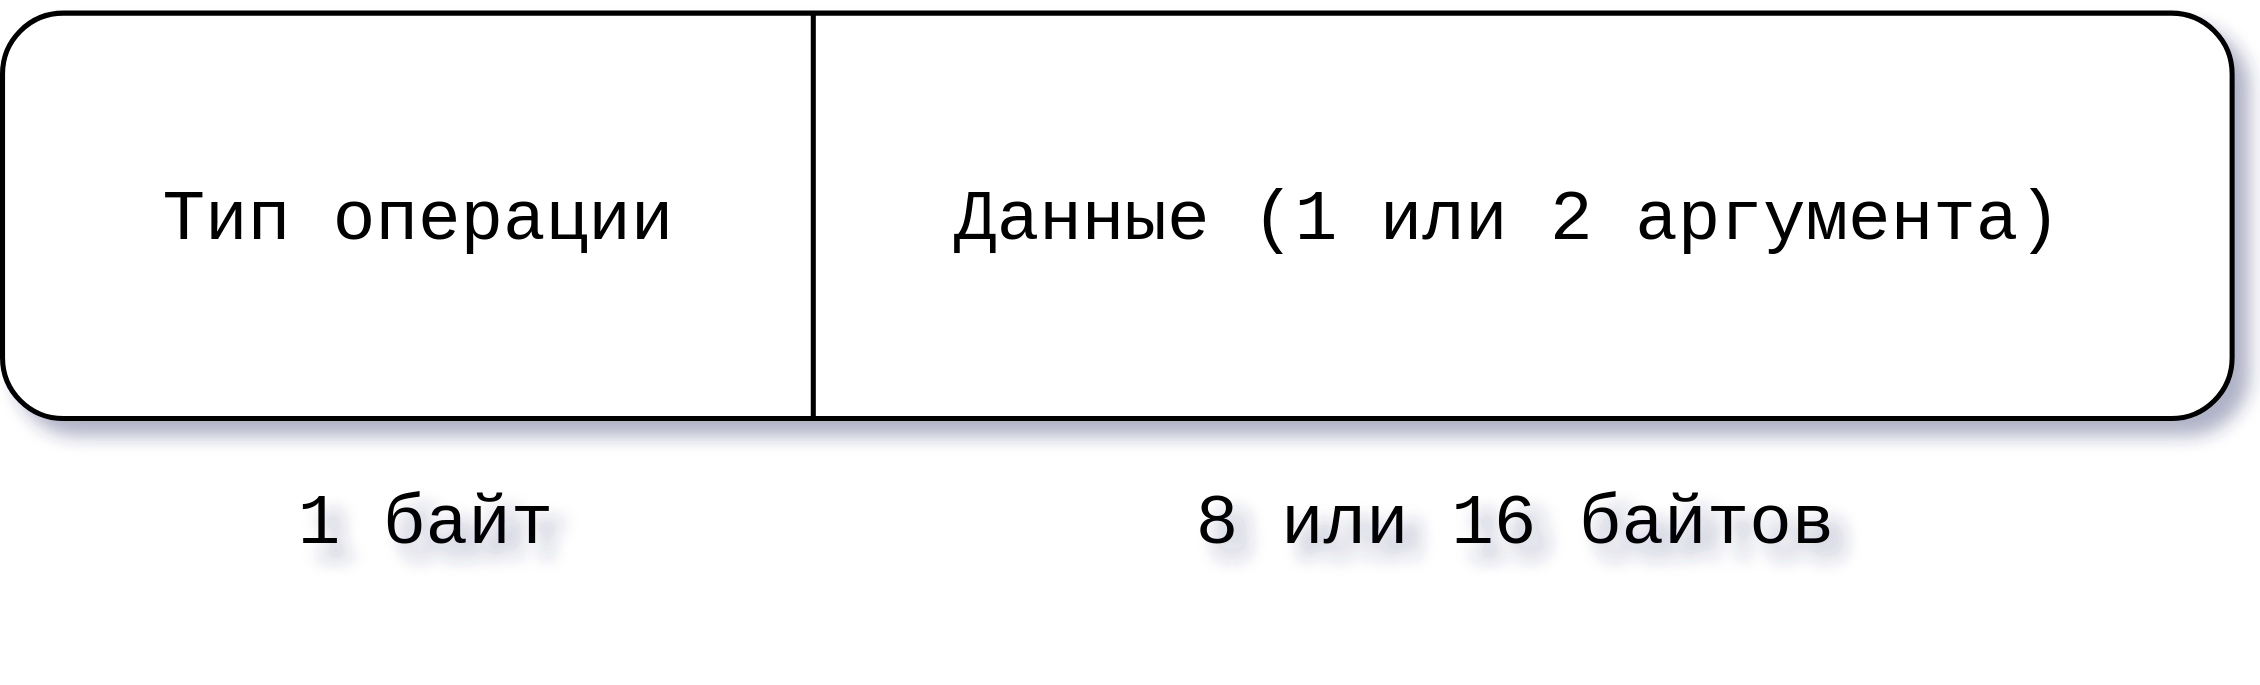
\includegraphics[width=0.8\textwidth]{MathOperation}
		\caption{Формат данных математического запроса}
		\label{fig:math-req}
	\end{figure}
	
	Данные разделены на 2 блока: тип операции, который занимает 1 байт, и данные (аргументы), которые занимают 8 байтов, если для данного типа операции необходим 1 операнд, или 16 байтов, если -- 2 операнда.
	
	В таблице \ref{tab:msg-types} представлены возможные типы операций, их бинарное представление и соответствующее количество аргументов.

	Операнды в бинарном виде кодируются <<старшими байтами вперёд>>.

	\begin{table}[H]
	\begin{center}
		\caption{Типы операций}
		\label{tab:msg-types}
		\def\tabcolsep{4pt}
		\begin{tabular}{|c|c|c|c|}
			\hline 
			& Тип операции & Бинарное представление & Число операндов \\ 
			\hline 
			1 & Сложение & $0000\text{ }0000$ & 2\\ 
			\hline 
			2 & Вычитание & $0000\text{ }0001$ & 2\\ 
			\hline 
			3 & Умножение & $0000\text{ }0010$ & 2\\ 
			\hline 
			4 & Деление & $0000\text{ }0011$ & 2\\ 
			\hline
			5 & Квадратный корень & $0000\text{ }0100$ & 1\\ 
			\hline 
			6 & Факториал & $0000\text{ }0101$  & 1\\ 
			\hline 
		\end{tabular} 
	\end{center}
	\end{table}
	
	\item \textbf{Ответ на математический запрос}.
	
	Данные для этого типа сообщения состоят из 2-х блоков: типа ответа, который кодируется 1 байтом, и численным результатом, который кодируется 8 байтами. Типы ответов, их бинарное представление и соответствующие значения численного результата приведены в таблице \ref{tab:math-resp}.
	
	\begin{table}[H]
	\begin{center}
		\caption{Типы ответов на математический запрос}
		\label{tab:math-resp}
		\def\tabcolsep{4pt}
		\fontsize{10}{11}\selectfont
		\begin{tabular}{|c|c|c|c|}
			\hline 
			& Тип ответа & Бинарное представление & Численный результат \\ 
			\hline 
			1 & Неправильная операция & $0000\text{ }0000$ & $0000\text{ }0000$\\ 
			\hline 
			2 & Результат на быструю операцию & $0000\text{ }0001$ & Вычисленное значение\\ 
			\hline 
			3 & <<Долгая>> операция была принята к вычислению & $0000\text{ }0010$ & $0000\text{ }0000$\\ 
			\hline 
		\end{tabular} 
	\end{center}
	\end{table}	

	2-й блок, в котором находится результат, заполняется 8-байтным числом-результатом матемаической операции, если тип ответа равен результату на быструю операцию, в остальных случаях заполняется нулём.	
	
		\item \textbf{Управляющий запрос запрос}.
		
		Данные для этого типа сообщения состоят из одного блока -- кода управляющего запроса, который кодируется 1 байтом. В настоящее время поддерживается 1 управляющий запрос -- запрос клиента на отключение себя. Ему соответствует код $0000\text{ }0000$.
	
		\item \textbf{Ответ на управляющий запрос запрос}.
		
		Данные для этого типа сообщения состоят из 1 блока -- кода ответа, который кодируется 1 байтом. В настоящее время ответ всегда 1 -- запрос на отключение прошёл успешно. Ему соответствует код $0000\text{ }0000$.
		
		\item \textbf{Запрос, инициируемый сервером} (он же результат вычисления <<долгой>> операции). Данные для этого типа сообщения состоят из 1 блока -- 8 байтов, которыми кодируется результат операции.
	
\end{enumerate}

\section{Реализация прикладного протокола}

Прикладной протокол реализован на языке \code{c++}. Рассмотрим основные абстракции, соответствующие компонентам прикладного протокола:

\begin{itemize}
	\item \code{TCP}
	
	Абстракцией самого верхнего уровня является класс \code{Message}. Он инкапсулирует в себе тип сообщения, которому соответствует перечисление \code{MessageType}, размер данных и сами данные в виде массива байтов. В зависимости от типа сообщения в качестве данных может быть либо байтовое представление объектов классов \code{Operation} и \code{MathResponse}, либо 1 байт для управляющего запроса и ответа на управляющий запрос, либо 8 байтов для результата выполнения <<долгой операции>>.
	
	Класс \code{Operation} является абстракцией для математического запроса --- математической операции, а класс \code{MathResponse} является абстракцией для ответа на математический запрос.
	
	\item \code{UDP}	
	
	Ввиду особенностей транспортного протокола \code{UDP}, в частности, отстутствия нумерации 	дэйтаграм, абстракцией самого верхнего уровня стал класс \code{NumberedMessage}, который инкапсулирует в себе номер сообщения и объект класса \code{Message}. В связи с другой особенностью \code{UDP} --- отсутствием подтверждения доставки дэйтаграмм, в перечисление \code{MessageType} был добавлен новый экземпляр, который имеет смысл \code{ACK} (подтверждения), изначально уже имеющегося в протоколе \code{TCP}.
	
\end{itemize}

\section{Описание архитектур приложений на основе \code{TCP} и \code{UDP}}
%приложений на основе TCP и UDP, их особенностей и ограничений (с графическими схемами

\subsection{Приложение на основе \code{TCP}}\label{sec:arch:tcp}

Архитектура приложения изображена на UML диаграмме компонентов на рис. \ref{fig:tcp-comp}.

\begin{figure}[H]
	\centering
	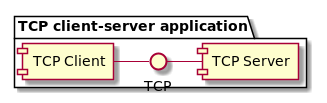
\includegraphics[width=0.8\textwidth]{TCPComponents}
	\caption{UML-диаграмма компонентов \code{TCP} приложения}
	\label{fig:tcp-comp}
\end{figure}

UML-диаграмма классов серверной части приложения представлена на рис. \ref{fig:tcp-classes}.

\begin{figure}[H]
	\centering
	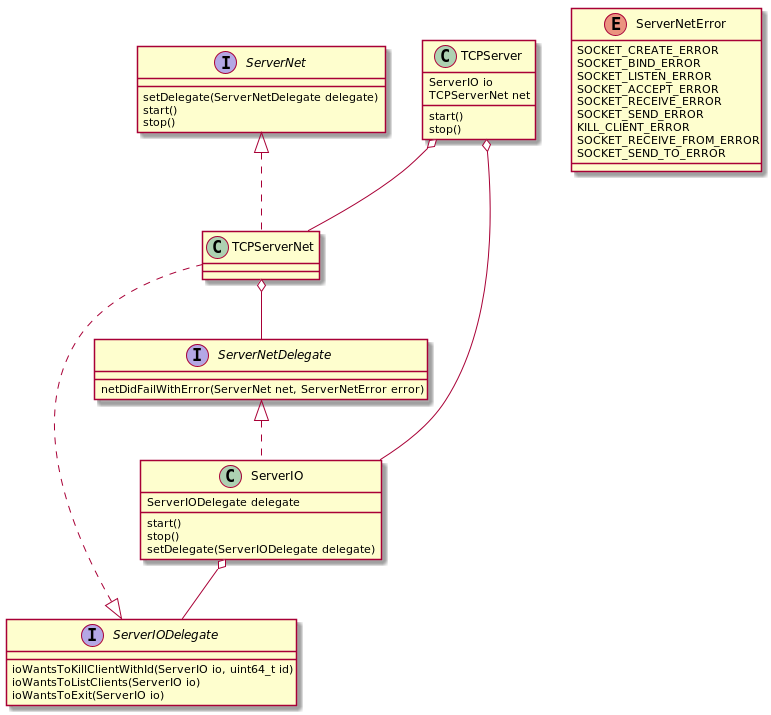
\includegraphics[width=1\textwidth]{TCPClasses}
	\caption{UML-диаграмма классов \code{TCP} сервера}
	\label{fig:tcp-classes}
\end{figure}

Класс \code{TCPServer} включает в себя два других --- \code{ServerIO} и \code{TCPServerNet}. \code{ServerIO} осуществляет взаимодействие с администратором через терминал, а также печатает в него возникающие ошибки.  В классе \code{TCPServerNet} реализована сетевая часть. 

При помощи паттерна проектирования Делегат, классы \code{ServerIO} и \code{TCPServerNet} взаимодейтсвуют друг с другом, реализуя соответственно интерфейсы 

\code{ServerNetDelegate} и \code{ServerIODelegate}.

Когда в классе \code{TCPServerNet} произошла сетевая ошибка или событие, о котором следует напечатать в консоль, он вызывает соответствующий метод \code{netDidFailWithError(ServerNet net, ServerNetError error)} своего делегата, которым является \code{ServerIO}.

Когда администратору сервера требуется вывести список обслуживаемых сервером клиентов, отключить какого-либо клиента или вовсе завершить работу сервера, он пишет команду в терминал, которая сначала принимается классом \code{ServerIO}, который затем вызывает методы

\code{ioWantsToKillClientWithId(ServerIO io, uint64\_t id)},

\code{ioWantsToListClients(ServerIO io)} и 
 
\code{ioWantsToExit(ServerIO io)} своего делегата, которым является \code{TCPServerNet}.\\[3mm]

Сервер поддерживает следующие консольные команды:

\begin{enumerate}
	\item \code{list} --- вывести список всех обслуживаемых клиентов в формате:\\ \code{ID. IP:PORT}
	\item \code{kill <client\_id>} --- отключить клиента с ID, равным <client\_id>
	\item \code{exit} --- завершить работу сервера
\end{enumerate}

Архитектура клиентской части приложения проста, и весь исходный код поместился в 1 файл.

Клиент поддерживает следующие консольные команды:

\begin{enumerate}
	\item \code{<A>+<B>} --- сложить числа \code{<A>} и \code{<B>}
	\item \code{<A>-<B>} --- вычесть из числа \code{<A>} число \code{<B>}
	\item \code{<A>*<B>} --- перемножить числа \code{<A>} и \code{<B>}
	\item \code{<A>\textbackslash<B>} --- разделить число \code{<A>} на число \code{<B>}
	\item \code{v<A>} --- извлечь квадратный корень из числа \code{<A>}
	\item \code{<A>!} --- вычислить факториал числа \code{<A>}
	\item \code{kill me} --- запрос к серверу на отключение
\end{enumerate}

\subsection{Приложение на основе \code{UDP}}\label{subsec:arch-udp}

Архитектура приложения изображена на UML диаграмме компонентов на рис. \ref{fig:udp-comp}.

\begin{figure}[H]
	\centering
	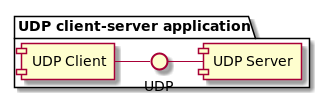
\includegraphics[width=0.8\textwidth]{UDPComponents}
	\caption{UML-диаграмма компонентов \code{UDP} приложения}
	\label{fig:udp-comp}
\end{figure}

UML-диаграмма классов серверной части приложения представлена на рис. \ref{fig:udp-classes}.

\begin{figure}[H]
	\centering
	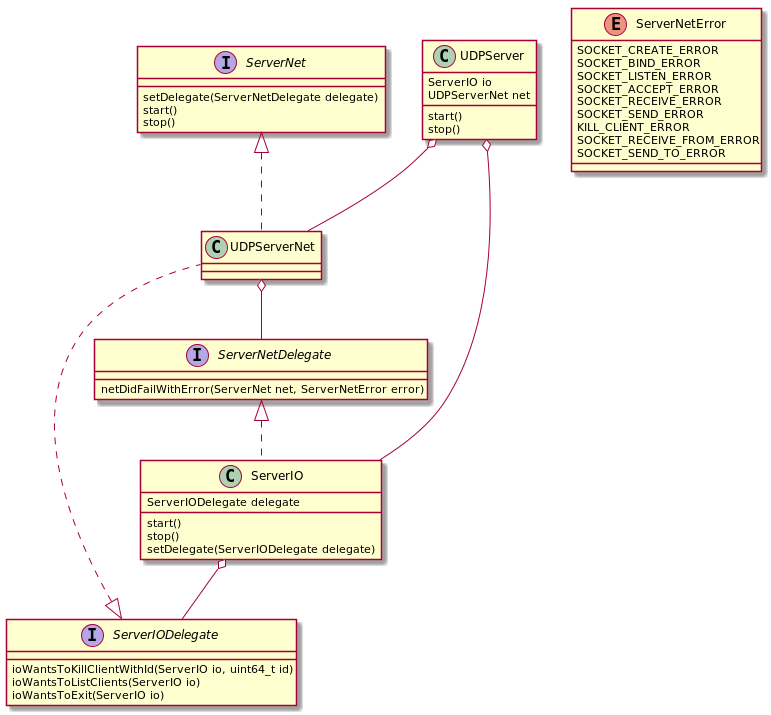
\includegraphics[width=1\textwidth]{UDPClasses}
	\caption{UML-диаграмма классов \code{UDP} сервера}
	\label{fig:udp-classes}
\end{figure}

В результате проектирования приложения на основе \code{TCP} получилась удачная архитектура (раздел \ref{sec:arch:tcp}), которая позволила при реализации \code{UDP} сервера разработать лишь классы \code{UDPServer} и \code{UDPServerNet}, которые являются заменой классам \code{TCPServer} и \code{TCPServerNet}. Другие отличия в архитектуре закрыты в реализациях \code{ServerNet} и будут рассмотрены в разделе \ref{sec:net}.\\[3mm]

Исходный код клиентской части \code{UDP} приложения состоит из одного класса --- \code{UDPClient}.\\[3mm]

Набор и формат консольных команд как в клиентской части, так и в серверной полностью совпадают с описанными в разделе \ref{sec:arch:tcp}.

\section{Особенности реализации сетевых и многопоточных приложений}\label{sec:net}

Все приложения были разработаны на языке \code{c++} с использованием некоторых возможностей стандарта \code{c++ 17}.

\subsection{Приложение на основе \code{TCP}}

При запуске серверного приложения главный поток порождает новый поток, в котором инстанс класса \code{ServerIO} осуществляет взаимодействие с администратором серверного приложения через консоль. Далее в главном потоке создаётся объект \code{TCPServerNet}, в котором устанавливается в режим прослушивания заданного порта сокет, созданный с помощью системной функции \code{socket()} с аргументами \code{AF\_INET}, \code{SOCK\_STREAM}, \code{IPPROTO\_TCP}. Затем в бесконечном цикле происходит вызов блокирующей системной функции \code{accept()}, которая возвращает дескриптор сокета для взаимодействия с клиентом в рамках новго соединения. Для взаимодействия с клиентом создается новый поток (<<клиентский>>). Каждому новому клиенту при помощи атомарной переменной типа \code{std::atomic<uint64\_t>} сопоставляется уникальный идентификатор. Данные о клиентах (идентификатор и дескриптор сокета) хранятся в переменной типа \code{std::unoredered\_map<uint64\_t, int>}, который является реализацией структуры данных хэш-таблица. Данная структура данных обеспечивает доступ к клиенту по идентификатору за время, независящее от количества хранимых в ней клиентов. В связи с тем, что доступ как на запись, так и на чтение к этой переменной  осуществляется из разных потоков, для синхронизации используется мютекс типа \code{std::shared\_mutex}, который позволяет потоку брать блокировку на чтение или на запись. Данная особенность мютекса позволяет осуществлять чтение хэш-таблицы с клиентами одновременно сразу нескольким потокам, в то время как записывать в один момент времени может лишь один поток. После выхода из бесконечного цикла, в котором происходит установление соединений с клиентами, сначала закрывается <<слушающий>> сокет, затем завершают свое выполнение все клиентские потоки, поняв, что <<слушающий>> сокет был закрыт. После этого закрываются клиентские сокеты и джойнятся клиентские потоки. В конце главный поток джойнит поток, в котором производилось взаимодействие с администратором приложения.

Рассмотрим подробнее взаимодействие сервера с клиентом. Со стороны сервера оно происходит в <<клиентском>> потоке. Сервер получает данные от клиента при помощи функции \code{readNBytes()}, которая реализована поверх системной функции \code{recv()}, и читает из сокета ровно то количество байтов, которое передано в неё в качестве аргумента. Если серверу пришёл запрос произвести <<быструю>> операцию, то выполнение операции и отправка клиенту ответа произойдёт в <<клиентском>> потоке. Если серверу пришёл запрос произвести <<долгую>> операцию, то в <<клиентском>> потоке он отправит ответ <<Долгая операция принята к выполнению>>, затем создаст новый поток, в котором выполнится эта <<долгая>> операция, и будет отправлен результат клиенту. В такой ситуации сервер выступает в роли клиента, а клиент --- в роли сервера. Для того, чтобы клиент мог асинхронно получать от сервера результаты <<долгих>> операций, не будучи заблокированным ожиданием ввода пользователем команды, у него есть 2 потока: в первом производится взаимодействие с пользователем через консоль и отправка серверу запросов, а во втором --- получение от сервера ответов.

\subsection{Приложение на основе \code{UDP}}

Как было сказано в разделе \ref{subsec:arch-udp}, отличие серверного приложения на основе протокола \code{UDP} от серверного приложения на основе \code{TCP} скрывается в реализации интерфейса (для \code{c++} -- класса, с полностью виртуальными методами) \code{ServerNet}. Поэтому рассмотрим класс \code{UDPServerNet}. В нём происходит создание главного сокета с помощью системной функции \code{socket()} с аргументами \code{AF\_INET}, \code{SOCK\_DGRAM}, \code{IPPROTO\_UDP}. Затем в бесконечном цикле происходит вызов функции \code{recvfrom()}. Данная функция помимо переданных клиентом данных отдаёт также стуктуру \code{sockaddr\_in}, которая содержит адрес клиентского приложения. Т.к. запросы от всех клиентов сервер получает через один сокет в одном потоке, для избавления от лишних задержек надо быстро определять, от кого получен запрос, и осуществлять обработку клиентского запроса в отдельном потоке. Для этого информация о всех клиентах на сервере хранится в хэш-таблице \code{std::unoredered\_map}, о скорости работы которой сказано в предыдущем разделе. После получения данных и адреса приложения клиента через вызов \code{recvfrom()} происходит быстрый поиск в хэш-таблице ключа --- адреса приложения клиента. Если он уже в ней содержится, значит уже был создан обработчик (объект класса \code{ClientHandler}), и нужно передать данные в него. Если такого ключа еще в хэш-таблице нет, то для такого ключа -- адреса приложения -- создается новый обработчик, и в него также передаются данные. Передача данных в обработчик является асинхронной и не блокирует поток, в котором происходит получение данных через сокет. Под <<вызовом обработчика>> подразумевается вызов метода \code{submit()} класса \code{ClientHandler}. Данный метод принимает в качестве аргументов данные в виде массива байтов, размер (число байтов) и 2 колбэка --- колбэк, в котором реализована отправка клиенту \code{ACK}, и колбэк, в котором реализована отправка клиенту ответа на запрос. Внутри метода \code{submit()} происходит обработка запроса в отдельном потоке, при этом в нужный момент вызываются колбэки. Использование двух колбэков в качестве аргументов метода \code{submit()} позволило всю работу с сетью (запись в сокет) оставить в классе \code{UDPServerNet}, а всю работу по обработке запросов --- внутри класса \code{ClientHandler}. По тому же принципу, что и в серверном приложении на основе \code{TCP}, хэш-таблица с данными о клиентах защищена мютексом \code{std::shared\_mutex}, а все потоки завершаются при закрытии сокета и джойнятся в родительском потоке. Для контроля перемешивания, пропадания или дублирования дэйтаграмм, в данных о каждом клиенте хранятся атомарные счётчики, позволяющие вести нумерацию сообщений. После получения от клиента запроса сервер отправляет клиенту \code{ACK}, а после отправки клиенту ответа --- ожидает от него \code{ACK}. Ожидание длится 1 секунду, затем сервер отправляет ответ снова. В итоге сервер может отправить до 10 ответов клиенту в случае неполучения \code{ACK}, а потом он перестаёт это делать.

Особенностью клиентского приложения является то, что если после отправки серверу запроса оно не получает от него \code{ACK} в течение 1 секунды, то оно посылает запрос снова. После 5-ти безуспешных попыток приложение информирует пользователя о проблеме и становистя готовым к отправке новых запросов.


\section{Результаты тестирования}
%приложения (с разным набором входных данных, методика тестирования параллельности обработки запросов клиентов, проверка программы на потерю, дублирование и перемешивание дейтаграмм) .

\section{Выводы}
%Анализ выполненных заданий, сравнение удобства/эффективности/количества проблем при программировании TCP/UDP. Если для реализации прикладного протокола поверх UDP потребовалась модификация прикладного протокола, упомянуть эти измнения. Области применения протоколов TCP и UDP

\end{document}
